\documentclass[a4paper, 12pt, french]{article}
\usepackage{ae,lmodern}
\usepackage[french]{babel}
\usepackage[utf8]{inputenc}
\usepackage[T1]{fontenc}
\usepackage[dvipsnames]{xcolor}
\usepackage{graphicx}
\usepackage{hyphenat}
\usepackage[left=15mm, right=15mm]{geometry}
\usepackage{csquotes}
\usepackage{bookmark}
\usepackage{biblatex}
\usepackage{listings}
\usepackage{hyperref}
\usepackage{eurosym}

\addbibresource{rapport.bib}

\lstset{
  aboveskip=3mm,
  belowskip=-2mm,
  backgroundcolor=\color{lightgray},
  basicstyle=\footnotesize,
  breakatwhitespace=false,
  breaklines=true,
  captionpos=b,
  commentstyle=\color{ForestGreen},
  deletekeywords={\ldots},
  escapeinside={\%*}{*)},
  extendedchars=true,
  framexleftmargin=16pt,
  framextopmargin=3pt,
  framexbottommargin=6pt,
  frame=tb,
  keepspaces=true,
  keywordstyle=\color{blue},
  language=Python,
  literate=
  {²}{{\textsuperscript{2}}}1
  {⁴}{{\textsuperscript{4}}}1
  {⁶}{{\textsuperscript{6}}}1
  {⁸}{{\textsuperscript{8}}}1
  {€}{{\euro{}}}1
  {é}{{\'{e}}}1
  {è}{{\`{e}}}1
  {ê}{{\^{e}}}1
  {ë}{{\¨{e}}}1
  {É}{{\'{E}}}1
  {Ê}{{\^{E}}}1
  {û}{{\^{u}}}1
  {ù}{{\`{u}}}1
  {â}{{\^{a}}}1
  {à}{{\`{a}}}1
  {á}{{\'{a}}}1
  {ã}{{\~{a}}}1
  {Á}{{\'{A}}}1
  {Â}{{\^{A}}}1
  {Ã}{{\~{A}}}1
  {ç}{{\c{c}}}1
  {Ç}{{\c{C}}}1
  {õ}{{\~{o}}}1
  {ó}{{\'{o}}}1
  {ô}{{\^{o}}}1
  {Õ}{{\~{O}}}1
  {Ó}{{\'{O}}}1
  {Ô}{{\^{O}}}1
  {î}{{\^{i}}}1
  {Î}{{\^{I}}}1
  {í}{{\'{i}}}1
  {Í}{{\~{Í}}}1,
  morekeywords={*,self, \_\_init\_\_, \_\_eq\_\_, \_\_str\_\_},
  numbers=left,
  numbersep=10pt,
  numberstyle=\tiny\color{black},
  rulecolor=\color{black},
  showspaces=false,
  showstringspaces=false,
  showtabs=false,
  stepnumber=1,
  stringstyle=\color{ForestGreen},
  tabsize=4,
  title=\lstname,
}

\title{
	\Huge
	\textbf{Application météo}
	\vspace{0.4cm}

	\LARGE
	Application Web et Sécurité
}

\author{
	Melissa Allaoua \\
        LE DENMAT Mickaël \\
        Hasnae Gaizi \\
        Gabriel Scrève \\Cambresy Florian \\
	Chalaud Jean-Christophe \\
	Le Denmat Mickael
}

\begin{document}
	\begin{titlepage}
    \begin{center}
        \vspace*{1cm}

        \Huge
        \textbf{Application météo}

        \vspace{0.4cm}
        \LARGE
        Application Web et Sécurité

        \vspace{1.6cm}

        \large
        Melissa Allaoua \\
        Mickaël Le Denmat \\
        Hasnae Gaizi \\
        Gabriel Scrève \\

        \vspace{10cm}

        
\includegraphics[width=0.32\textwidth]{images/UVSQ-logo}

        \vspace{0.4cm}

        \Large
        Université de Versailles Saint-Quentin-en-Yvelines \\
        \vspace{0.4cm}
        15 Mai 2022
    \end{center}
\end{titlepage}

	\newpage
	\renewcommand{\contentsname}{Table des matières}
	\tableofcontents

	\newpage
	\section{Application météo}
		Notre projet est une application météo. Elle affiche les
		informations classiques des applications météo comme
		une petite discription de la météo, la température,
		le ressenti, la vitesse du vent, \ldots
		Elle affiche aussi la températeur de la ville toute les trois heures,
		et la météo sur sept jours.
		
		\scalebox{.33}{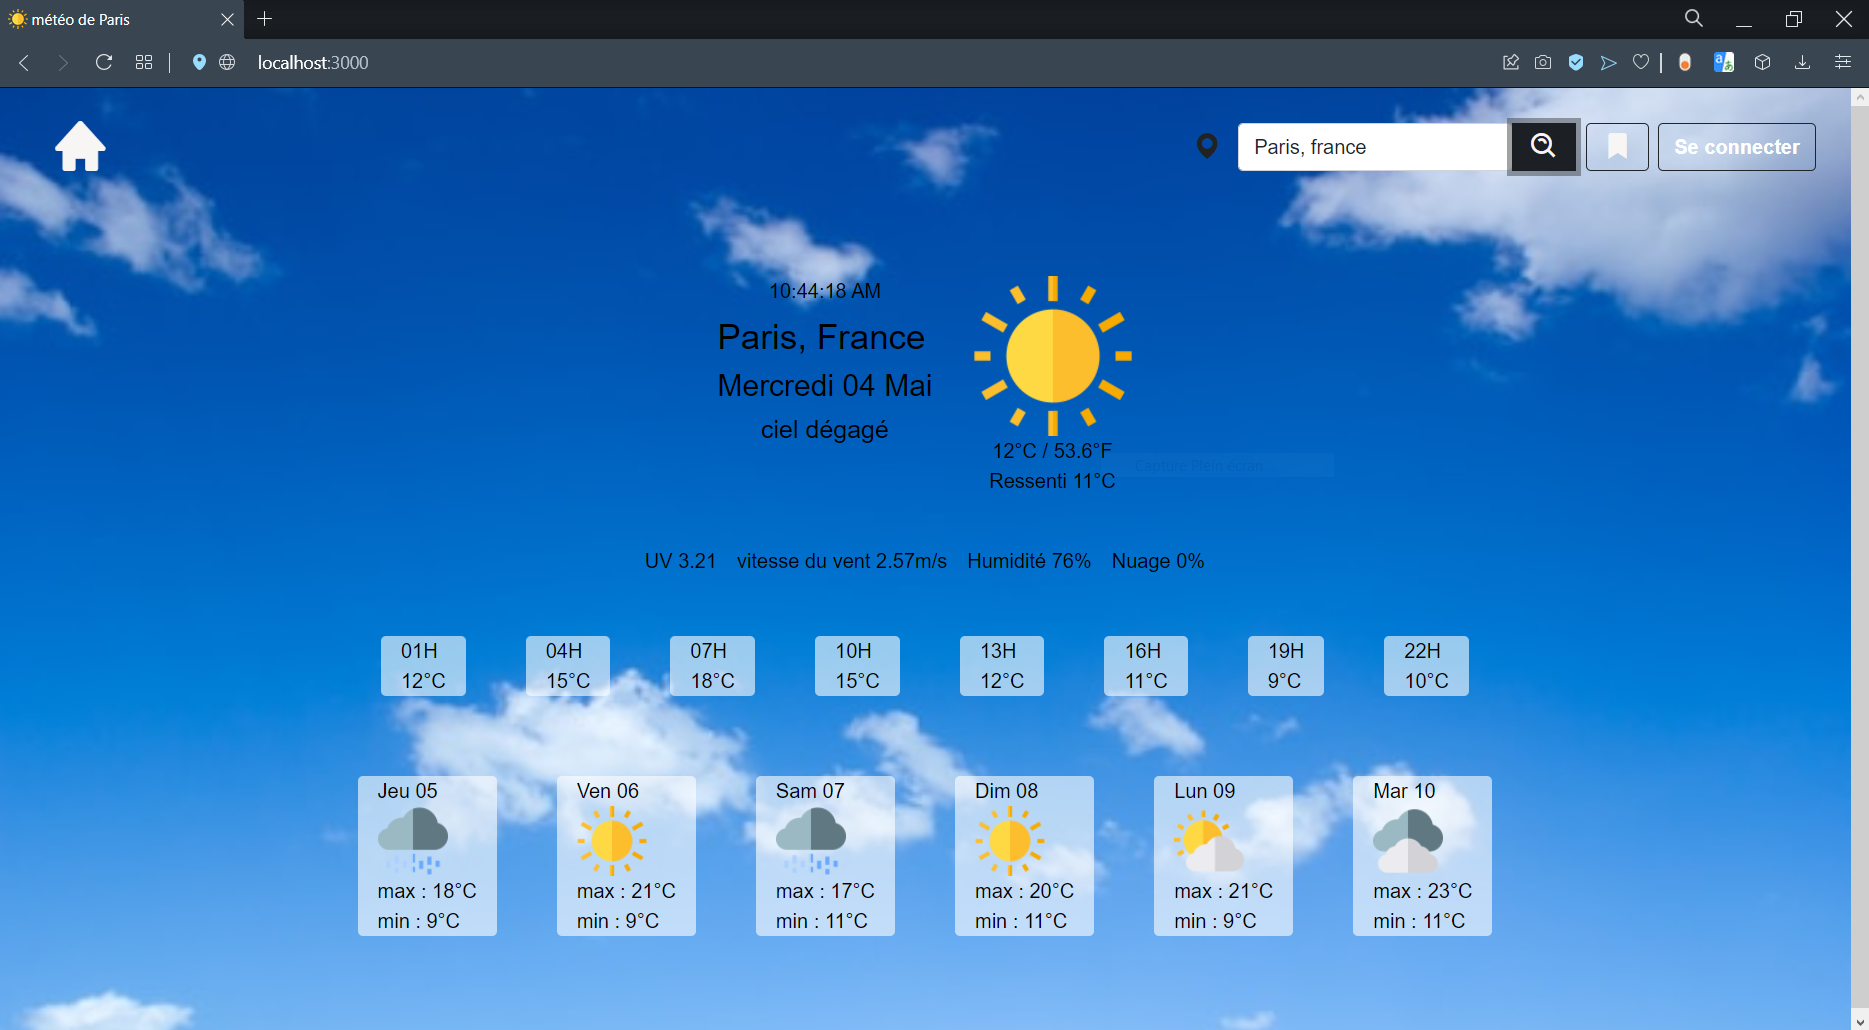
\includegraphics{images/app-meteo.PNG}}

		L'utilisateur a la possibilité de se connecter pour acceder à ses
		favoris, c'est-à-dire des villes qu'il a mis en favoris afin de
		voir la météo de ses villes sans les cherchers.

	\section{Technologie(s) utilisée(s)}
		\subsection{Bootstrap}
			Bootstrap est un framework css \cite*{Bootstrap} utilisé pour construire des sites
			réactif aux différentes tailles d'écrans ainsi que des sites pour les
			téléphones.

			Nous l'avons utilisé afin d'organiser rapidement et facilement
			les éléments au sein de notre application, c'est-à-dire les grilles,
			les espaces, les couleurs, \ldots

			Le site de Bootstrap propose aussi beaucoup d'exemples 
			\cite*{Bootstrap-Exemples}. Nous avons en copié certains
			pour avoir une base fonctionnelle que nous avons modifié pour
			ajouter ce dont nous avons besoin et que cela sois dans le même
			style que notre application.

			Beaucoup de framework existe mais Bootstrap, étant la plus connue, a plus de
			documents, de tutoreils Youtube ou autre et plus d'aide sur les forums en cas de
			bug. Lors du developpement de l'application, Bootstrap a parfaitement
			collé à nos besoin, nous n'avons pas eu besoin de trouvé une autre bibliothéque.

		\subsection{OpenWeatherApp}
			OpenWeatherApp est site proposant des services concernant la météo. Il permet
			de faire des requêtes à ces différentes API's pour connaître la météo, actuelle
			ou heure par heure, les prévisions de la semaine, l'humidité, l'uv, \ldots
			\cite*{OpenWeatherApp}.

			Nous utilisons une de leur API appelé OneCall \cite*{OpenWeatherApp-OneCall}
			qui nous permet d'obtenir toutes les informations essentiels en un seul appel.
			Nous récupèrons un json avec la météo actuelle, une prévision de la météo pour
			les sept jours a venir, une prévision pour les heurs a venir. L'appel a l'API se
			fait comme cela :\url{https://api.openweathermap.org/data/2.5/onecall?lat=
			{lat}&lon={lon}&exclude={part}&appid={API key}}.

			Ensuite nous utilisons une variante de cette dernière afin d'avoir les informations
			concernant la météo des heures passées. Pour cela nous faisons appel à 
			\url{https://api.openweathermap.org/data/2.5/onecall/
			timemachine?lat={lat}&lon={lon}&dt={time}&appid={API key}}.

			Avec ces deux API's nous avons toutes les informations nécéssaires à notre projet.

		\subsection{Express et NodeJS}

		\subsection{}

	\section{Quelques points importants}
	\section{Structure}

	\printbibliography

\end{document}
